\documentclass[11pt]{article}
\usepackage{tikz}


\author{Andrew}
\date{text }

\begin{document}
\begin{center}
CPSC 413 Assignment 1 \\
by Andrew Garcia-Colrey
\end{center}
\section{Problem 1}
Question 1
\begin{center}
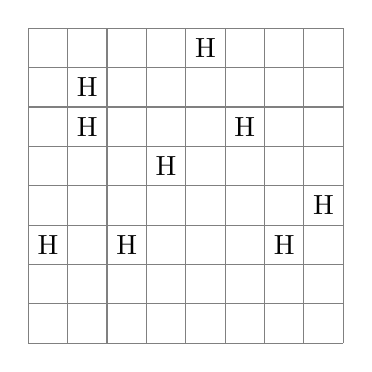
\begin{tikzpicture}
\draw[step=0.5cm,color=gray] (-1,-1) grid (3,3);
\node at (1.25,+2.75) {H};
\node at (-.25,+2.25) {H};
\node at (-0.25,+1.75) {H};
\node at (+0.75,+1.25) {H};
\node at (1.75,+1.75) {H};
\node at (2.75,+0.75) {H};
\node at (+2.25,0.25) {H};
\node at (+.25,+0.25) {H};
\node at (-.75,.25) {H};
\end{tikzpicture}
\end{center}
Question 2
\hfill \break
\break
Two ways to look at this problem is to either minimize the amount of houses that are visited, or to maximize the amount of house each Mailmen finds. In my search for an algorithm I began debating between two main Algorithms I will refer to as \textbf{Shortest}  and \textbf{Most Houses}. 
\hfill \break
\break
\textbf{Shortest} simply starts by looking both down and right and checks to see from the current position of the mailman which one is closer and takes a step in that direction. then proceeds to checks again by looking down and to the right to see if there is a house closer to himself now that he has moved in on of the two directions.
\hfill \break
\break
 \textbf{Most Houses} works in a similar fashion the previous Algorithm by looking in both directions. However where this Algorithm differ is that instead of looking for closest House, it instead looks for the most amount of Houses in that direction regardless of how far away it is. then upon moving in the direction with the most houses, the Algorithm then repeats the previous check by looking in both directions to ensure that.
 \hfill \break
\break
However upon further examination and counter example exploration the  \textbf{Most Houses} fails to give an optimal solution for the following graph

\noindent\fboxsep{%
\begin{minipage}{14em}
 \centering
 Figure 1
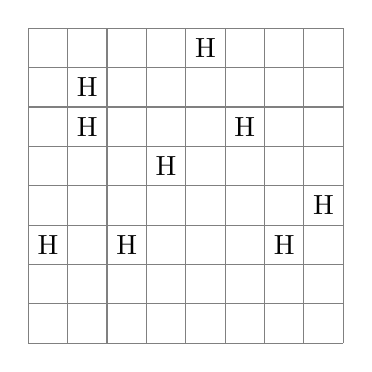
\begin{tikzpicture}

\draw[step=0.5cm,color=gray] (-1,-1) grid (3,3);
\node at (1.25,+2.75) {H};
\node at (-.25,+2.25) {H};
\node at (-0.25,+1.75) {H};
\node at (+0.75,+1.25) {H};
\node at (1.75,+1.75) {H};
\node at (2.75,+0.75) {H};
\node at (+2.25,0.25) {H};
\node at (+.25,+0.25) {H};
\node at (-.75,.25) {H};
\end{tikzpicture}
\end{minipage}}%
\hfill%
\fboxsep{%
\begin{minipage}{14em}
 \centering
 Figure 2
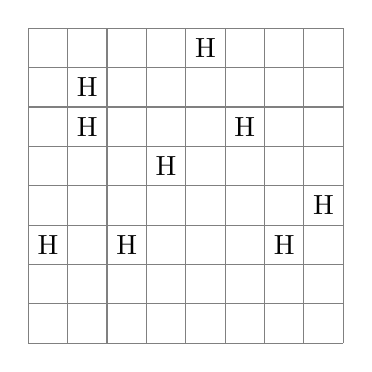
\begin{tikzpicture}

\draw[step=0.5cm,color=gray] (-1,-1) grid (3,3);
\node at (1.25,+2.75) {H};
\node at (-.25,+2.25) {H};
\node at (-0.25,+1.75) {H};
\node at (+0.75,+1.25) {H};
\node at (1.75,+1.75) {H};
\node at (2.75,+0.75) {H};
\node at (+2.25,0.25) {H};
\node at (+.25,+0.25) {H};
\node at (-.75,.25) {H};
\end{tikzpicture}
\end{minipage}
}





\hfill \break
\break
Where as the Shortest path method still gives the optimal number of paths which is 3. This does not mean that our  \textbf{Shortest} Algorithm is correct 
 


\pagebreak

Question 2.1
\begin{center}

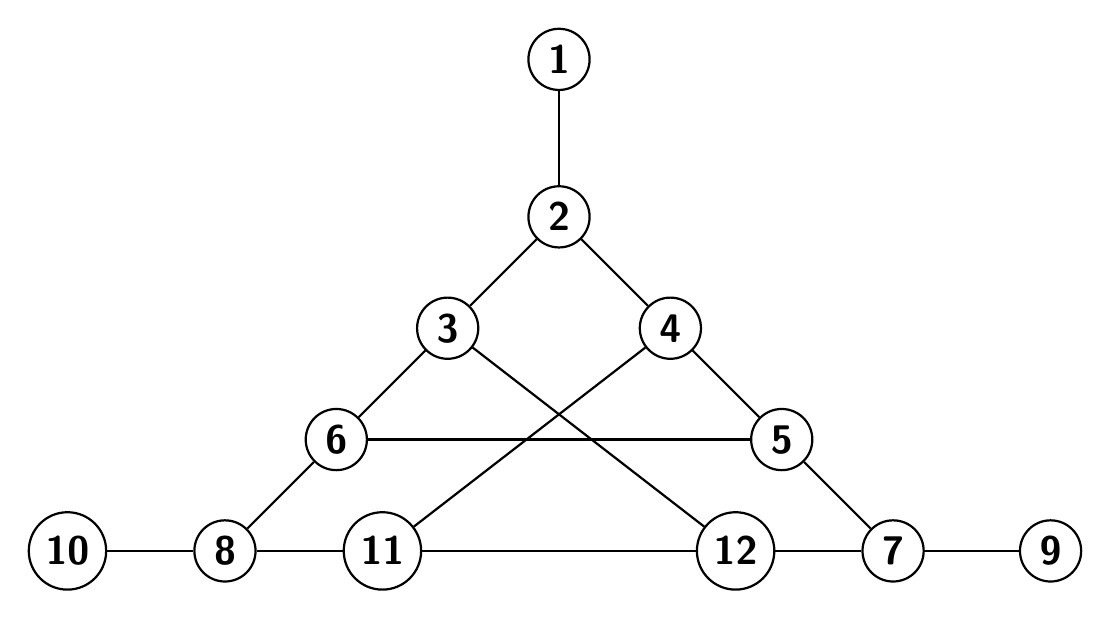
\begin{tikzpicture}[auto, node distance=2cm, every loop/.style={},
                    thick,main node/.style={circle,draw,font=\sffamily\Large\bfseries}]

  \node[main node] (1) {1};
  \node[main node] (2) [below of=1] {2};
  \node[main node] (3) [below  left of=2] {3};
  \node[main node] (4) [below  right of=2] {4};
  \node[main node] (5) [below  right of=4] {5};
  \node[main node] (6) [below  left of=3] {6};
  \node[main node] (7) [below  right of=5] {7};
  \node[main node] (8) [below  left of=6] {8};
  \node[main node] (9) [  right of=7] {9};
  \node[main node] (10) [  left of=8] {10};
  \node[main node] (11) [  right of=8] {11};
  \node[main node] (12) [  left of=7] {12};
         
         
\path[every node/.style={font=\sffamily\small}]
    (1) edge node [left] {} (2)
    (2) edge node [right] {} (4)
    (2) edge node [right] {} (3)
    (3) edge node [right] {} (6)
    (6) edge node [right] {} (8)
    (4) edge node [right] {} (5)
     (5) edge node [right] {} (7)
      (7) edge node [right] {} (9)
       (10) edge node [right] {} (8)
        (8) edge node [right] {} (11)
         (11) edge node [right] {} (12)
          (12) edge node [right] {} (7)
          (3) edge node [right] {} (12)
          (4) edge node [right] {} (11)
          (6) edge node [right] {} (5);
    
   
    
  

  

 
\end{tikzpicture}
\end{center}
\pagebreak
Question 2.2
\\
\\
\begin{center}
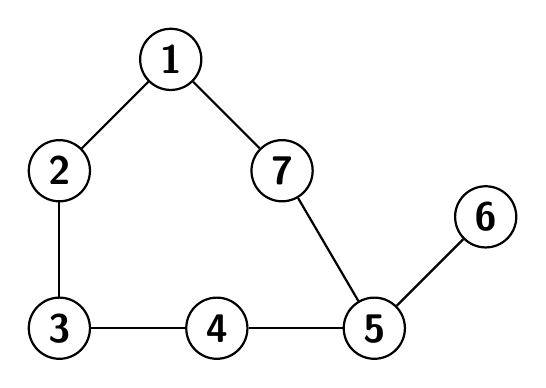
\begin{tikzpicture}[auto, node distance=2cm, every loop/.style={},
                    thick,main node/.style={circle,draw,font=\sffamily\Large\bfseries}]

  \node[main node] (1) {1};
  \node[main node] (2) [below left of=1] {2};
\node[main node] (3) [below  of=2] {3};
\node[main node] (4) [right  of=3] {4};
\node[main node] (5) [ right  of=4] {5};
\node[main node] (6) [above right  of=5] {6};
\node[main node] (7) [below right  of=1] {7};


\path[every node/.style={font=\sffamily\small}]
    (1) edge node [left] {} (2)
    (2) edge node [left] {} (3)
    (3) edge node [left] {} (4)
    (4) edge node [left] {} (5)
    (5) edge node [left] {} (6)
    (5) edge node [left] {} (7)
    (7) edge node [left] {} (1);

    
         

  

  

 
\end{tikzpicture}
\end{center}

Question 2.3
\\
\\
\begin{center}
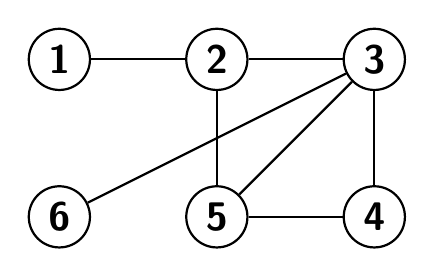
\begin{tikzpicture}[auto, node distance=2cm, every loop/.style={},
                    thick,main node/.style={circle,draw,font=\sffamily\Large\bfseries}]

  \node[main node] (1) {1};
  \node[main node] (2) [ right of=1] {2};
    \node[main node] (3) [ right of=2] {3};
      \node[main node] (4) [ below of=3] {4};
        \node[main node] (5) [ left of=4] {5};
          \node[main node] (6) [ left of=5] {6};

\path[every node/.style={font=\sffamily\small}]
    (1) edge node [left] {} (2)
    (2) edge node [left] {} (3)
    (3) edge node [left] {} (4)
    (4) edge node [left] {} (5)
   
    (3) edge node [left] {} (5)
    (6) edge node [left] {} (3)
    (2) edge node [left] {} (5);

    
         


    
         

  

  

 
\end{tikzpicture}
\end{center}




\end{document}